\section{Pure-Shift Spectra via \acl{2DJ} Estimation}
\label{sec:pure-shift}

Two key features which the \ac{NMR} community is constantly seeking to improve
are the sensitivity and resolving power of experiments. There are
numerous means of improving spectral sensitivity, via technological
advancements including the production of superconducting magnets with higher
field strengths\note{CITE?} (sensitivity $\propto B_0^{\nicefrac{7}{4}}$),
and cryogenic probes\cite{Kovacs2005}, as well as simply increasing the number
of scans (\ac{SNR} $\propto \text{NS}^{\nicefrac{1}{2}}$).  There are however
few means of achieving better resolution beyond increased field strengths
(resolution $\propto B_0$). Significant interest has therefore been
given to the development of homodecoupled (``pure shift'')
experiments\cite{Meyer2013,Adams2014,Zangger2015}, in which the
effects of homonuclear scalar couplings are removed from the data. The presence
of J-couplings, indicating the close proximity of spins in a chemical
bonding sense, is a distinguishing feature of \ac{NMR}, and is often valuable for
structural assignment. However, in many cases their effect can lead to spectra
which are too crowded for meaningful insights to be gleamed.  Heteronuclear
couplings, between spins with different nuclei (i.e. \proton\ and \carbon) are
straightforward to decouple at the point of \ac{FID} acquisition, using well
known schemes such as WALTZ-16\cite{Shaka1983a, Shaka1983b} and
GARP\cite{Shaka1985}. Homonuclear decoupling is anything but simple on the
other hand.

In this section, an overview of the key techniques which have
been developed to generate pure shift spectra is given, starting with \ac{2DJ}
spectroscopy and finishing up with \ac{PSYCHE}, widely considered the most
robust pure shift experiment in terms of sensitivity and tolerance to strong
coupling. Subsequently, a new technique for generating pure shift spectra via
parametric estimation, named \acf{CUPID} is presented.

\subsection{An Overview of Pure Shift NMR}

\subsubsection{The \acl{2DJ} Experiment}
The \ac{2DJ} experiment\cite{Aue1976, Morris2009} provided the first means of
achieving pure shift spectra.  It has a simple pulse sequence, presented in
Figure \ref{fig:pure_shift_seqs}.a: after excitation of magnetisation onto the
transverse plane, the indirect dimension evolution consists of a spin echo, with
acquisition following immediately afterwards. Fourier transformation in both
dimensions leads to a spectrum in which only scalar couplings contribute in
$\Fone$, as the chemical shifts are refocussed by the spin echo, while both
scalar couplings and chemical shifts contribute in $\Ftwo$.
Peaks belonging to a particular multiplet lie along a line at \ang{45} to the
$F^{(1)}$ and $F^{(2)}$ axes, as seen in panel a. of Figure
\ref{fig:jres_spectrum}.
\begin{figure}%
    \centering%
    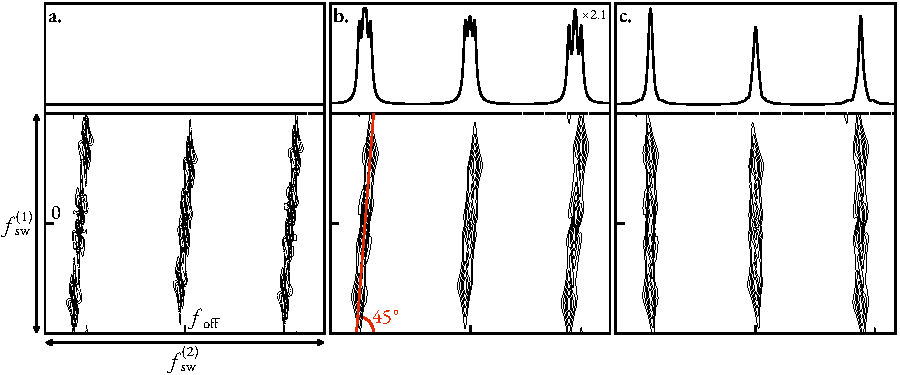
\includegraphics{jres_spectrum/jres_spectrum.pdf}%
    \caption{%
        \textbf{a.} Contour plot \ac{2DJ} absolute value mode spectrum for an
        AMX spin system, produced by applying sine-bell apodisation on a hypercomplex
        \ac{FID} before a \ac{FT} in both dimensions. Each multiplet lies a
        long a line at \ang{45} to the $F^{(1)}$ and $F^{(2)}$ axes. Note that
        this line often appears to make an angle that is greater than \ang{45}
        with the $F^{(2)}$ axis when viewing spectra, since typically $\fswone
        \ll \fswtwo$. Above the \ac{2DJ} spectrum is a plot of its summation
        along the $\Fone$ axis.
        \textbf{b.} Spectrum generated after application of a \ang{45} shear,
        with its $\Fone$ summation above.
   }%
    \label{fig:jres_spectrum}%
\end{figure}%

An FID generated by the \ac{2DJ} experiment is hypercomplex, taking the form of
\eqref{eq:general fid} with $D=2$ and $\zeta = \exp(\iu\cdot)$, i.e.
\begin{equation}%
    \begin{split}%
        \jresfid\idxnonentwo =
        \sum_{m=0}^{M-1} \bdam \exp\left( \iu \bdphim \right)
            \exp\left(\left(2 \pi \iu \bdfonem - \bdetaonem\right) {\none}_{\vphantom{t}} \Dtone\right) \times \\
            \exp\left(\left(2 \pi \iu \bdftwom - \bdetatwom\right) {\ntwo}_{\vphantom{t}} \Dttwo\right)
            + \symbf{W}\left[n^{(1)}, n^{(2)}\right].
    \end{split}%
    \label{eq:jres-fid}
\end{equation}%
A major downside of the \ac{2DJ} experiment is there is no means of generating
a pair of phase- or amplitude-modulated signals which are the
conventional route to frequency-discriminated spectra with absorption mode
lineshapes. In many multidimensional experiments, changing the phase of
certain \ac{RF} pulses or the use of \acp{PFG} can induce a change in the \ac{CTP},
generating such signal-pairs, though this unavailable with \ac{2DJ}
spectroscopy as no mixing time exists. The FT of $\jresfid$ produces a spectrum
$\jresspec$ with ``phase-twist'' peaks, which possess contributions from both absorption
and dispersion Lorentzians. There are two primary steps involved in obtaining a
pure shift spectrum from $\jresspec$:
\begin{enumerate}
    \item Perform a \ang{45} shear (often called a tilt) on the spectrum array,
        leading to the separation of chemical shifts and scalar couplings onto
        orthogonal axes  (panel b. in Figure \ref{fig:jres_spectrum}). Each
        slice in $\Ftwo$ is subjected to a right circular rotation such that
        \begin{subequations}
            \begin{gather}
                \jresspectilt\left[{\none}\vpsub{\mathrm{sw}},{\ntwo}\vpsub{\mathrm{sw}}\right] =
                \jresspec\left[{\none}\vpsub{\mathrm{sw}},\ntwonew\right],\\
                \ntwonew = \left(
                    {\ntwo}\vpsub{\mathrm{new}} + \left\lfloor
                        \frac
                            {\fswone \Ntwo\vpsub{\mathrm{sw}}}
                            {\fswtwo \None\vpsub{\mathrm{sw}}}
                        \left(
                            \frac{\None\vpsub{\mathrm{sw}}}{2} - \none
                        \right)
                    \right\rceil
                \right) \bmod \Ntwo.
            \end{gather}
        \end{subequations}
        This achieves the mapping $\jresspec\left(\fone,\ftwo\right)
        \rightarrow \jresspec\left(\fone, \ftwo - \fone\right)$.  It should be
        noted that the effectiveness of the shear is maximised when both
        $\nicefrac{\fswtwo}{\fswone}$ and $\nicefrac{\Ntwo}{\None}$ are powers
        of 2\note{check this}.
    \item Sum the spectrum along $\Fone$:
        \begin{equation}
            \specps\idxntwo =
            \sum_{\none=0}^{\None-1} \jresspectilt\idxnonentwo.
        \end{equation}
\end{enumerate}%
Shearing and summing $\jresspec$ actually leads to the absorptive and dispersive
components of the spectrum cancelling each other out . It is necessary to display
the spectrum in absolute value mode before carrying out the above steps (i.e.
use $\Re(\lvert \jresspec \rvert)$).
This still leads to undesirable pure shift spectra with broad ``wings'' on
account of the presence of dispersive character. The dispersive component can
be suppressed by appropriate processing to make the FID envelope symmetric in
both dimensions, such as with sine-bell
apodisation\cite[Section3.3.5]{Lindon1980}, or pseudo-echo
reshaping\cite{Bax1981}, though this results in a significant reduction in
sensitivity being incurred.

\begin{figure}
    \centering
    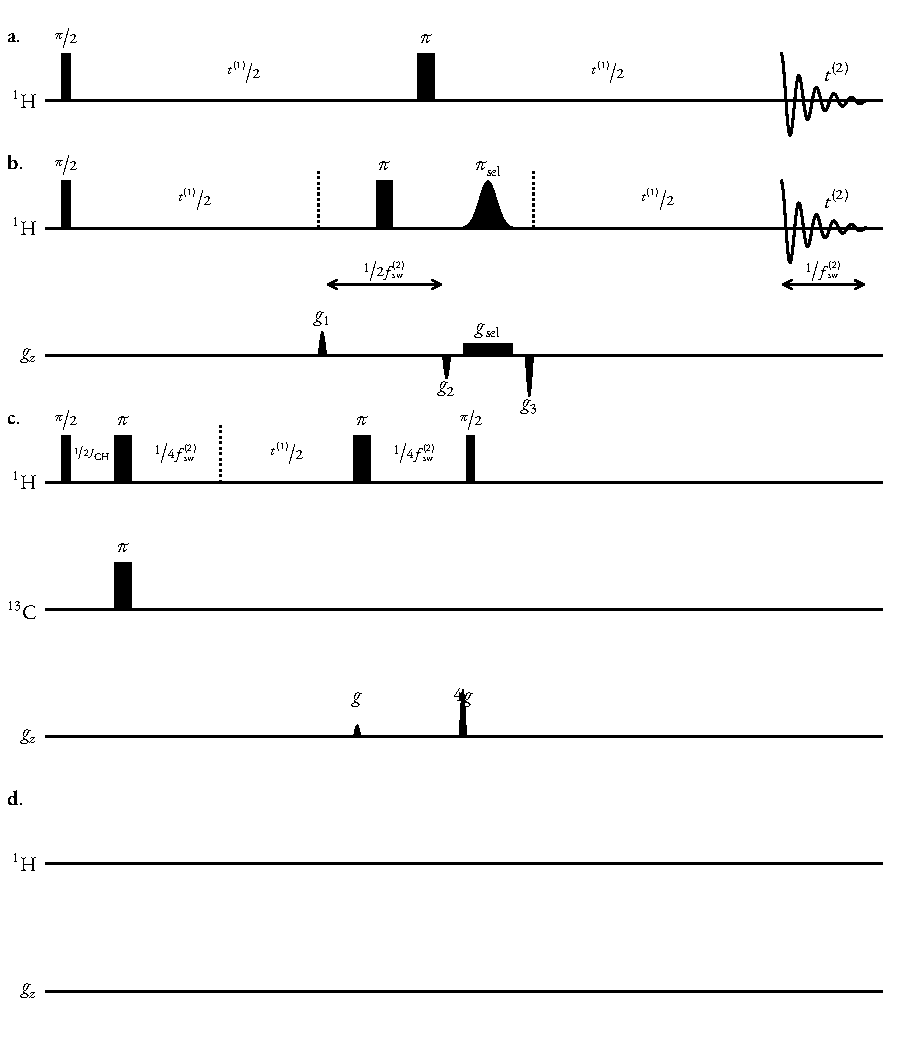
\includegraphics{pure_shift_sequences/pure_shift_sequences.pdf}
    \caption{
        \note{Work needed. Figure out the correct delays in ZS, BIRD, PSYCHE}
        The pulse sequences of four of the most common pure shift experiments.
        \textbf{a.} \acs{2DJ}.
        \textbf{b.} The \acs{ZS} method.
        \textbf{c.} The \acs{BIRD} method.
        \textbf{d.} The \acs{PSYCHE} method.
    }
    \label{fig:pure_shift_seqs}
\end{figure}

\subsubsection{The \acl{ZS} Method}
\label{subsec:ZS}
In 1997 Zangger and Sterk introduced a pulse sequence element which achieves
slice-selective excitation, by applying a low \ac{RF} power (weak) \ang{180}
pulse\footnote{Conventionally, a R-SNOB pulse is used\cite{Kupce1995}.} in the
presence of a \ac{PFG} along the $z$-axis\cite{Zangger1997}. Such an element
excites a
given spin only in a narrow range of heights in the sample, as the \ac{PFG}
induces a shift in resonance frequency according to $\Delta \omega(z) = \gamma
G_z z$, where $G_z$ is the magnitude of the \ac{PFG}. By placing a hard
\ang{180} pulse adjacent to the selective pulse, the
``active'' spin in a given slice is rotated by \ang{360} (i.e. no net
rotation), while all other (``passive'') spins are only rotated by \ang{180}.
Placing such a element in the middle of the $\tone$ evolution therefore
achieves refocussing of the J-couplings associated with the active
spin\cite{Aguilar2010}. In order to achieve effective decoupling of any given
pair of spins, it is necessary that the bandwidth of the selective π-pulse is
smaller than the difference in their chemical shifts. However, with more
selective pulses, a smaller proportion of the available spin magnetisation will
contribute to the final FID, and hence sensitivity will be diminished
\footnote{
    The reduction in sensitivity is $\propto \nicefrac{f_B}{\gamma G_z l_z}$,
    where $f_B$ is the selective pulse bandwidth, and $l_z$ is the length of
    the sample lying within the receiver coil ($\approx
    \qty{1.5}{\centi\meter}$).
}.
There is therefore a trade-off between effective decoupling of all spins, and
achieving the greatest sensitivity possible. In the case of strong coupling,
the \ac{ZS} method tends to perform poorly relative to other options for this
reason. The \ac{ZS} element has been applied by Keeler and Pell in order to
generate \ac{2DJ} datasets comprising phase-modulated pairs, enabling the
generation of pure absorption-mode spectra\cite{Pell2007}.


\subsubsection{The \acs{BIRD} Method}
The \ac{BIRD} pulse sequence element\cite{Garbow1982,Bax1983}, presented in
Figure \ref{fig:pure_shift_seqs}.c, also takes advantage of the idea of
selectively inverting passive spins, while leaving active spins unaffected.
However the active spins are those which are directly bound to
\textsuperscript{13}C nuclei, which naturally occur with an abundance of 1.1\%,
while the passive spins are those bound to far more abundant
\textsuperscript{12}C nuclei. The reduction in sensitivity of the experiment
relative to a full-sensitivity experiment is therefore known and constant
across samples. In scenarios where is this strong coupling, \ac{BIRD} can
achieve improved sensitivity over \ac{ZS}, since with the latter a very weak
selective pulse would be required to ensure it is of a sufficiently small
bandwidth. The \ac{BIRD} method is particularly attractive in scenarios where
the sensitivity penalty due to the involvement of a low-abundance nucleus has
already been paid, for example in a \ac{HSQC} experiment\cite{Paudel2013}.

\subsubsection{PSYCHE}
\label{subsec:psyche}
\note{TODO}
Original paper\cite{Foroozandeh2014}, tutorial paper\cite{Foroozandeh2018}, PSYCHE-2DJ\cite{Kiraly2017}.

\subsubsection{Pure Shift NMR via J-Resolved Post-Processing}

There have been previous descriptions of acquiring pure-shift spectra from
typical \ac{2DJ} datasets via more sophisticated post-processing methods.
Nuzillard presented \ac{ALPESTRE}\cite{Nuzillard1996}, in which the parameters
of each indirect-dimension FID are estimated using linear prediction, such that
there is a set of parameters $\symbf{\Theta} \in \mathbb{R}^{\Ntwo \times 4M}$
with
\begin{equation}
    \symbf{\Theta}\left[\ntwo\right] =
    \begin{bmatrix}
        \left[\bda_{\ntwo}\right]\T &
        \left[\bdphi_{\ntwo}\right]\T &
        \left[\bdfone_{\ntwo}\right]\T &
        \left[\bdetaone_{\ntwo}\right]\T
    \end{bmatrix}.
\end{equation}
The parameters generated are used to propagate each FID backward into
$-\tone$, producing a ``full-echo'':
\begin{equation}
    \begin{split}
        \symbf{Y}_{\text{full}}\left[\none, \ntwo\right] = \sum_{m=0}^{M-1}
            \bda_{\ntwo} \left[ m \right]
            \exp\left(\iu \bdphi_{\ntwo} \left[ m \right] \right)
            \exp\left(\left(2 \pi \iu \bdfone_{\ntwo} \left[ m \right] \none
            -\bdetaone_{\ntwo} \left[ m \right] \left\lvert \none \right\rvert \right)\Dtone\right) \\
        \forall \none \in \mathbb{Z}: -\None < \none < \None,\\ \forall \ntwo \in \mathbb{N}_0: \ntwo < \Ntwo.
    \end{split}
\end{equation}
\ac{FT} of generates a spectrum whose real component comprises absorption-mode
Lorentzian character in both dimensions. This opens up the means of producing
pure-shift spectra from the \ac{2DJ} experiment with sharp lineshapes and
without sensitivity loss. A similar approach proposed by Mutzenhardt et al.
instead constructed full echoes via \ac{LP} of each direct-dimension
\ac{FID}, and generation of a full echo by propagating
into $-\ttwo$\cite{Mutzenhardt1999}.

\subsection{An outline of \acs{CUPID}}
\ac{CUPID} aims to generate pure shift spectra by utilising the result of
parametric estimation on \ac{2DJ} data, assumed to take the functional form of
\eqref{eq:jres-fid}.
Instead of estimating successive \ac{1D} \acp{FID}, as has been described by
Nuzillard and Mutzenhardt et al., the entire \ac{2DJ} signal is estimated as a
whole, giving access to the parameter vector $\bth \in \mathbb{R}^{6M}$. Using
$\bth$, a synthetic \ac{1D} \ac{FID}, named the ``\ang{-45} signal'' (Figure
\ref{fig:neg-45}), is produced:
\begin{equation}
    \symbf{y}_{\ang{-45}}\left(\bth\right)\left[ \ntwo \right] =
        \sum_{m=0}^{M-1} \bdam \exp \left(\iu \bdphim \right)
        \exp\left(
            \left(
                2 \pi \iu \left(\bdftwom - \bdfonem\right)
                - \bdetatwom
            \right) \ntwo \Dttwo
        \right).
    \label{eq:neg-45}
\end{equation}
$\forall \ntwo \in \lbrace 0, \cdots, \Ntwo - 1 \rbrace$. The \ang{-45} signal
takes the same functional form as a typical \ac{1D}
\ac{FID} acquired by a pulse-acquire experiment, except that the frequency of
each oscillator, which would usually be $\ftwo$, is replaced with $\ftwo -
\fone$. In a \ac{2DJ} experiment, $\fone$ corresponds to the displacement of a
given oscillator from the central frequency of the multiplet it is associated
with. As such, the oscillators belonging to a given multiplet all provide
a contribution with the same frequency to the \ang{-45} signal, namely the
chemical shift of relevant spin.
\begin{figure}
    \centering
    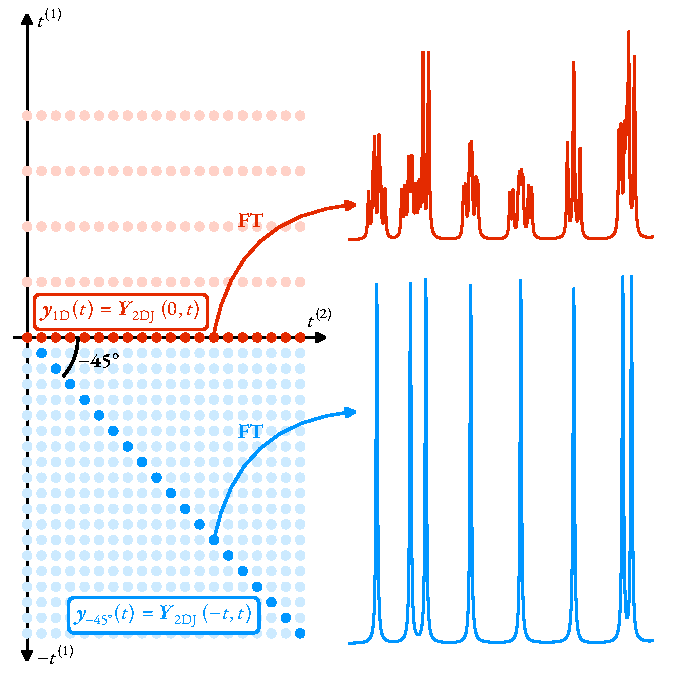
\includegraphics{neg_45_signal/neg_45_signal.pdf}
    \caption{
        An illustration of the reasoning behind the name ``\ang{-45}
        signal''. The pale red dots denote a typical \ac{2DJ} \ac{FID}, where
        the amount and rate of sampling in the direct dimension is greater than
        in the indirect dimension (i.e. $\None \ll \Ntwo$ and $\fswone \ll
        \fswtwo$). The bright red dots correspond to the first direct-dimension
        signal $\bY_{\text{2DJ}}(0, \ttwo)$, which has the same form as
        \iac{FID} from a pulse-acquire experiment. A hypothetical signal
        generated by propagating the \ac{FID} into $-\tone$, with the same rate
        of sampling in both dimensions, is denoted with pale blue dots. Taking
        the diagonal of this signal, such that it forms a \ang{-45} to the
        $\ttwo$ axis, yields an \ac{FID} $\by_{\ang{-45}}$  which is
        homodecoupled. It should be noted that there is a slightly discrepancy
        between \eqref{eq:neg-45} and this description, in that the
        indirect-dimension damping factors $\bdetaone$ are neglected in the
        former case.
    }
    \label{fig:neg-45}
\end{figure}

\subsubsection{Multiplet Prediction}
A holistic \ac{2D} estimation of the \ac{FID} provides access to other useful
information about the dataset. One such example is the grouping of oscillators
in account of which multiplet structure they belong to. As has already been
established, for oscillators which are associated with the same multiplet
structure, the quantity $\ftwo - \fone$ should be equal. This provides a
criterion in order to assess whether it is likely that two oscillators in the
estimation result belong to the same multiplet:
\begin{equation}
    \left \lvert
        \left( \bdftwo \left[ m_1 \right] -
        \bdfone \left[ m_1 \right] \right) -
        \left( \bdftwo \left[ m_2 \right] -
        \bdfone \left[ m_2 \right] \right)
    \right \rvert < \epsilon
\end{equation}
$\forall m_1, m_2 \in \lbrace 0, \cdots, M-1 \rbrace$, with  $\epsilon \in
\mathbb{R}_{>0}$ being a suitable threshold to account for error in the
estimation. An appropriate value for $\epsilon$ would appear to be half the
spectral resolution in the more poorly resolved dimension ($\Fone$), i.e.
$\epsilon = \nicefrac{\fswone}{2 \None}$. In situations involving real \ac{2DJ}
signals however, it is found that $\epsilon$ sometimes has to be increased to
values slightly larger than this to achieve effective groupings (\textit{vide
infra}). Algorithm \ref{alg:mp-assign} provides a routine that can be used for
multiplet prediction.

\note{Removal of spurious oscillators}

\subsubsection{Filtration of \ac{2DJ} data}
Unlike the direct-dimension, which can often comprise sparsely distributed
peaks in the Fourier domain, the indirect dimension of \ac{2DJ} datasets tends
to be rather densely populated. As such, it is typically of little use in
attempting to generate filtered sub-\acp{FID} in the indirect dimension. The
filtering procedure utilised for \ac{2DJ} data is therefore an extension of the
filtration procedure for \ac{1D} data described in Section \ref{sec:filtering}
(Figure \ref{fig:jres-filtering}). The filtering procedure involves the
following steps:
\begin{enumerate}
    \item The signal $\symbf{Y}_{\text{ve}} \in \mathbb{C}^{\None \times 2 \Ntwo}$ is
    constructed, such that a virtual echo is formed from each direct-dimension
    signal:
    \begin{equation}
        \begin{split}
            \symbf{Y}_{\text{ve}} \left[n^{(1)}\right] =
                &\left[
                \begin{matrix}
                    \Re\left(\symbf{Y}\left[n^{(1)}, 0\right]\right) &
                    \symbf{Y}\left[n^{(1)}, 1\right] &
                    \cdots
                \end{matrix}\right.
                \\
                &\left.
                \begin{matrix}
                    \symbf{Y}\left[n^{(1)}, \Ntwo - 1\right] &
                    0 &
                    \symbf{Y}\left[n^{(1)}, \Ntwo - 1\right]^* &
                    \cdots &
                    \symbf{Y}\left[n^{(1)}, 1\right]^*
                \end{matrix}
                \right]
        \end{split}
    \end{equation}
    $\forall n^{(1)} \in \lbrace 0, \cdots, N^{(1)} - 1 \rbrace$.
    \item $\symbf{Y}_{\text{ve}}$ is subjected to \ac{FT} along the direct
        dimension to produce the spectrum  $\symbf{S}_{\text{ve}}$ (panel a of
        Figure \ref{fig:jres-filtering}). This has a imaginary component of
        zeros.
    \item A super-Gaussian $\symbf{G} \in \mathbb{R}^{\None \times 2 \Ntwo}$ is
        constructed (panel b):
        \begin{equation}
            \symbf{G} = \symbf{1} \otimes \symbf{g}^{(2)},
        \end{equation}
        where $\symbf{1} \in \mathbb{R}^{\None}$ is a vector of ones, and
        $\symbf{g}^{(2)}$ is a super-Gaussian vector given by
        \eqref{eq:super-Gaussian-onedim} with $d=2$.
    \item A matrix of additive noise is generated by extracting the variance
        $\sigma^2$ of a strip of $\symbf{S}_{\text{ve}}$ which is devoid of
        peaks, and generating an array $\symbf{W}_{\sigma^2} \in
        \mathbb{R}^{\None \times 2 \Ntwo}$ with values independently sampled
        from a normal distribution with mean $0$ and variance  $\sigma^2$.
    \item The spectrum is filtered according to \eqref{eq:Sve-tilde}, yielding
        $\widetilde{\symbf{S}}_{\text{ve}}$ (panel d).
    \item $\widetilde{\symbf{S}}_{\text{ve}}$ is subjected to \ac{IFT} and is
        slicing in half in the direct dimension, yeilding the final filtered
        signal $\widetilde{\symbf{Y}}$:
        \begin{equation}
            \widetilde{\symbf{Y}} = \IFT^{(2)}\left(\widetilde{\symbf{S}}_{\text{ve}}\right) \left[:, : \Ntwo\right].
        \end{equation}
\end{enumerate}

\begin{figure}
    \centering
    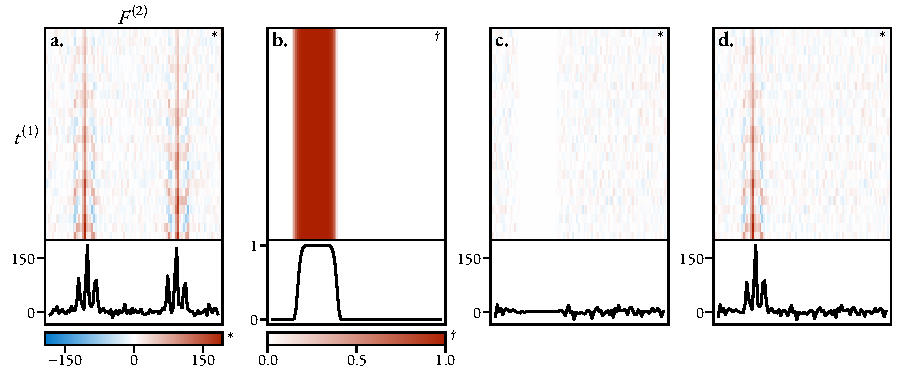
\includegraphics{jres_filtering/jres_filtering.pdf}
    \caption{
        An illustration of the filtering procedure for \ac{2DJ} data.
        For each panel is a heat-map of the full \ac{2D} signal, as well as a
        plot underneath of the first slice of the signal in the direct
        dimension.
        \textbf{a.} The spectrum $\symbf{S}_{\text{ve}}$,
        \textbf{b.} Super-Gaussian filter $\symbf{G}$,
        \textbf{c.} Additive noise, attenuated by the super-Gaussian, $\symbf{W}_{\sigma^2} \odot (\symbf{1} - \symbf{G})$,
        \textbf{d.} Filtered spectrum $\widetilde{\symbf{S}}_{\text{ve}}$
        Panels \textbf{a.}--\textbf{d.} are analogous to panels \textbf{b.}--
        \textbf{e.} in Figure \ref{fig:filtering} for the \ac{1D} case.
    }
    \label{fig:jres-filtering}
\end{figure}

\subsection{Results Using \acs{CUPID}}
A number of examples of the application of \ac{CUPID} are now provided.
Initially, a few results are presented using data simulated using the Spinach
MATLAB\textregistered\ library\cite{Hogben2011}. After this, examples are
provided with experimental data. In a couple of these, comparison of the result
acquired using \ac{CUPID} is compared with a spectrum acquired using
\ac{PSYCHE}.

\subsubsection{``Four Multiplets''}
\begin{figure}
    \centering
    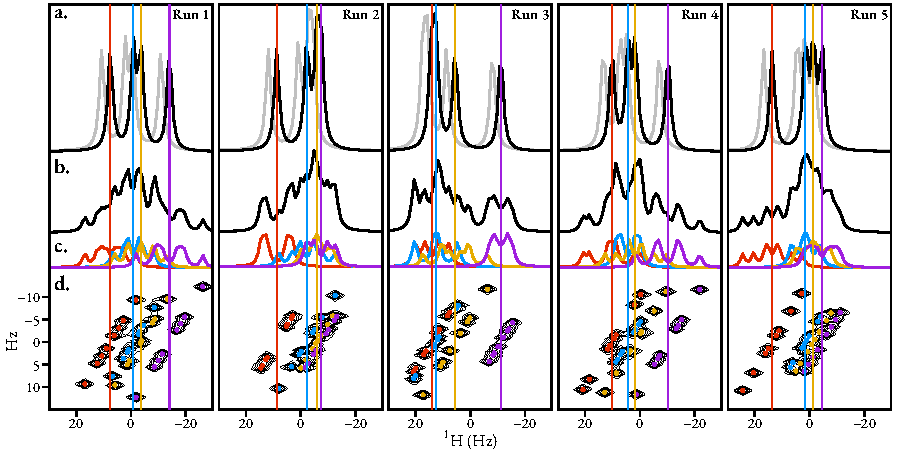
\includegraphics{four_multiplets/four_multiplets}
    \caption[
        The result of applying \ac{CUPID} to 5 instances of simulated \ac{2DJ}
        datasets with 4 heavily overlapping multiplet structures.
    ]{
        The result of applying \ac{CUPID} to 5 instances of simulated \ac{2DJ}
        datasets with 4 heavily overlapping multiplet structures.
        \textbf{a.} Black: pure shift spectrum generated by \ac{CUPID}.
        Grey: \ac{1D} spectrum simulated with Spinach, using the same spin
        system as was used to produce the \ac{2DJ} dataset, but with all scalar
        couplings sets to \qty{0}{\hertz}. This has been offset slightly for
        clarity.
        \textbf{b.} \ac{1D} spectrum of the dataset.
        \textbf{c.} Multiplet structures predicted, using a threshold $\epsilon
        = \nicefrac{\fswtwo}{\Ntwo}$.
        \textbf{d.} Contour plot of the \ac{2DJ} spectrum in absolute-value
        mode. Coloured points denote the frequencies of oscillators in the
        estimation result.
        Coloured vertical lines denote the predicted central frequencies of
        each multiplet structure.
    }
    \label{fig:four-multiplets}
\end{figure}
A series of simulated \proton\ \ac{2DJ} datasets were generated such that
within a known region of the spectrum, four ddd multiplet structures with
significant overlap existed. To achieve this, a spin-system with 7 spins was
formed, with the spins divided into 2 subsets:
\begin{itemize}
    \item 4 of the spins (the ``estimated spins'') were assigned random
        resonance frequencies sampled from $\mathcal{U}(\qty{-20}{\hertz},
        \qty{20}{\hertz})$.
    \item The remaining 3 spins (the ``coupling spins''), were coupled to each
        of the estimated spins, with the values of the couplings randomly
        sampled from $\mathcal{U}(\qty{-10}{\hertz}, \qty{10}{\hertz})$.  The
        coupling spins were given chemical shifts such that they lay far from
        the estimated spins in the spectrum (i.e. their frequencies were $\gg
        \qty{20}{\hertz}$).
\end{itemize}
\ac{AWGN} noise was added to the \ac{FID}, with a target \ac{SNR} of \qty{30}{\deci\bel}.
A filtered sub-\ac{FID} containing only the signals from the estimated spins
was then generated using the filtering procedure described above, with
$l^{(2)}_{\unit{\hertz}} = \qty{30}{\hertz}$,
$r^{(2)}_{\unit{\hertz}} = \qty{-30}{\hertz}$, and
$\xi = 1.1$. The resulting sub-\ac{FID} was expected to comprise 32 ($4 \times
2^3$) oscillators. To assess the estimation procedure's ability, a random
integer from the range 33 -- 40 was selected as the initial number of
oscillators. Hence, the initial guess from the \ac{MMEMPM} would comprise an
excessive number of oscillators. The \ac{FID} was subjected to
estimation, yielding the result vector $\bthstar$. Spurious oscillators were
checked for, using the criteria outlined above, with the threshold for
multiplet assignment set to the spectral resolution in the direct dimension:
$\epsilon = \nicefrac{f_{\text{sw}}^{(2)}}{\Ntwo}$.  If spurious oscillators
were found, these were removed, and \ac{NLP} was run on the updated set of
parameters.

Figure \ref{fig:four-multiplets} illustrates the result achieved for 5 separate
runs of the procedure described above \note{Table of shifts and couplings in the
appendix}.  For each \ac{FID} generated, the method was effective at producing an
estimation result with 32 oscillators, as desired, despite the excessive number
that were present in $\bthzero$. Most of the excessive oscillators were purged
from $\bthzero$ through the \ac{NLP} procedure. When spurious oscillators did
remain\footnote{for 2 of the 5 datasets, the result after \ac{NLP} comprised 33
oscillators}, they were then detected when checking for spurious oscillators
and subsequently removed. The pure-shift spectra generated using \ac{CUPID}
closely agree with pure-shift spectra generated by running a Spinach simulation
on a spin system with the same chemical shifts, but with all scalar couplings
set to \qty{0}{\hertz}.

\subsubsection{``Sucrose''}

\subsubsection{Quinine}
\begin{figure}
    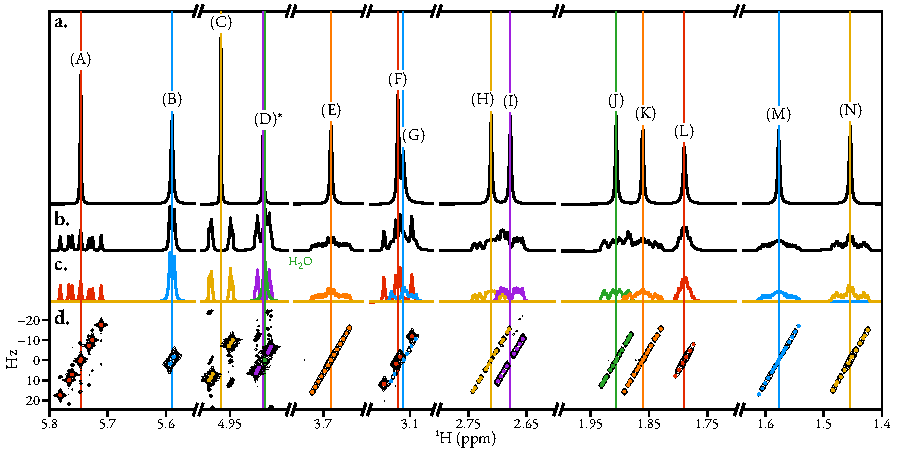
\includegraphics{quinine_cupid/quinine_cupid.pdf}
    \caption{TODO}
    \label{fig:quinine-cupid}
\end{figure}
